% =======================
% Chapter: Sentence Embedding Algorithms
%
% Author: Daniel Wehner
%

% -----------------------------------------------------------------------------------------------------------------------------------------------------
\section{Sentence Embedding Algorithms}
\label{sec:sent_embs}

\vspace*{-0.5mm}
% -----------------------------------------------------------------------------------------------------------------------------------------------------
% Chapter Introduction
\subsection{Introduction}
\label{sec:sent_embs_intro}

Due to the significant impact word embeddings had on the performance of machine learning techniques in the context of \gls{nlp}, the question arose whether it is possible to encode even larger spans of text in terms of a single vector. \citep{Le.2014} were among the first researchers to introduce embeddings for sentences, paragraphs and even entire documents. This chapter gives an introduction to common sentence embedding algorithms. \citep{Yang.2018} distinguish between two major approaches: They differentiate between \textbf{non-parameterized} methods which combine underlying word embeddings and \textbf{parameterized} methods which train sentence embeddings from scratch. Table \vref{tab:sent_embs_types} gives an overview of common algorithms (\textit{not exhaustive}):

% Table: Types and examples of sentence embeddings
\vspace*{3mm}
\begin{table}[h]
	\centering
	\renewcommand{\arraystretch}{1.4}
	\scalebox{0.95}{
	\begin{tabularx}{\textwidth}{| X | l ? X | l |}
		\hline
		\multicolumn{2}{| c ?}{
			\cellcolor{tud9c!50}
				\textbf{Non-parameterized methods}}				&
		\multicolumn{2}{ c |}{
			\cellcolor{tud9c!50}
				\textbf{Parameterized methods}} 					\\
		\rowcolor{tud9c!30}
		\textbf{Algorithm} 										&
		\textbf{Source} 											&
		\textbf{Algorithm} 										&
		\textbf{Source}											\\
		\hline\hline

		\ding{182} \textit{Vanilla average}							&
		\textit{- no author found -}								&
		\ding{182} \textit{Skip-Thought} 							&
		\citep{Kiros.2015} 									\\
		\hline

		\ding{183} \textit{Concatenated $p$-means}				&
		\citep{Rueckle.2018}										&
		\ding{183} \textit{Quick-Thought}							&
		\citep{Logeswaran.2018}									\\
		\hline

		\ding{184} \textit{\gls{gem}}		 						&
		\citep{Yang.2018} 										&
		\ding{184} \textit{sent2vec}								&
		\citep{Pagliardini.2018}									\\
  		\hline

		\ding{185} \textit{\gls{sif}}	 							&
		\citep{Arora.2017}										&
		\ding{185} \textit{InferSent} 								&
		\citep{Conneau.2017} 									\\
  		\hline

		\cellcolor{lightgray!50}		 							&
		\cellcolor{lightgray!50}		 							&
		\ding{186} \textit{\gls{sbert}} 								&
		\citep{Reimers.2019} 										\\
  		\hline

		\cellcolor{lightgray!50}		 							&
		\cellcolor{lightgray!50}		 							&
		\ding{187} \textit{\gls{laser}} 								&
		\citep{Artetxe.2018} 										\\
  		\hline
	\end{tabularx}}
	\caption[Types and examples of sentence embedding algorithms]
	{Types and examples of sentence embedding algorithms.
		Non-parameterized methods combine existing word embeddings to obtain a sentence representation
		whereas parameterized methods train sentence embeddings from scratch.}
	\label{tab:sent_embs_types}
\end{table}
\vspace*{3mm}

The rest of this chapter is organized as follows: Section \vref{sec:sent_embs_non_param} introduces some examples of non-parameterized algorithms which are going to be used in the experiments. Section \vref{sec:sent_embs_param} then presents their parameterized counterparts. Analogously to the previous chapter, details are given where and how the individual sentence encoders were obtained (cf. section \vref{sec:sent_embs_acquisition} for more information).

% -----------------------------------------------------------------------------------------------------------------------------------------------------
% Non-parameterized Sentence Embeddings
\subsection{Non-parameterized Sentence Embeddings / Compositional Models}
\label{sec:sent_embs_non_param}

\vspace*{-1mm}
% -----------------------------------------------------------------------------------------------------------------------------------------------------
% Vanilla Average
\subsubsection{Vanilla Average}
\label{sec:vanilla_average}

The most straightforward approach to generate a sentence representation is the \textit{vanilla average} technique. The embeddings of the words in the sentence to be encoded are averaged using a simple \textbf{arithmetic mean}: $\bm{v}_s = \frac{1}{T} \sum_{t=1}^T \bm{v}_{w_t}$, where $T$ denotes the length of the sentence. While this approach is very intuitive and easy to implement, it has severe shortcomings: \ding{182} It \textbf{neglects the word order}, therefore it is also referred to as a \gls{bow} approach. \ding{183}\,Furthermore, \textbf{stop-words and more informative words are weighted equally} \citep{Le.2014}. Figure \vref{fig:mean_sentence_embedding} shows an exemplary sentence:

% Figure: Example for mean sentence embeddings
\begin{figure}[h]
	\centering
	\begin{tikzpicture}[
		scale=0.7,
		every node/.style={scale=0.7},
		arr/.style={stealth-stealth,double}
	]

		\node at (-3,0) {\Large $w_t$};
		\node (w1) at (0,0) {\strut\large\textbf{One}};
		\node (w2) at (3,0) {\strut\large\textbf{ring}};
		\node (w3) at (6,0) {\strut\large\textbf{to}};
		\node (w4) at (9,0) {\strut\large\textbf{rule}};
		\node (w5) at (12,0) {\strut\large\textbf{them}};
		\node (w6) at (15,0) {\strut\large\textbf{all}};
		\node (w7) at (18,0) {\strut\large\textbf{.}};

		\node at (-3,-3) {\Large $\bm{v}_{w_t}$};
		\node (v1) at (0,-3) {$\begin{bmatrix} 5.04 \\ -3.45 \\ \vdots \\ 0.06 \end{bmatrix}$};
		\node (v2) at (3,-3) {$\begin{bmatrix} 0.34 \\ 1.08 \\ \vdots \\ -5.87 \end{bmatrix}$};
		\node (v3) at (6,-3) {$\begin{bmatrix} -0.05 \\ 2.46 \\ \vdots \\ -1.34 \end{bmatrix}$};
		\node (v4) at (9,-3) {$\begin{bmatrix} -7.83 \\ 0.27 \\ \vdots \\ 3.36 \end{bmatrix}$};
		\node (v5) at (12,-3) {$\begin{bmatrix} -8.92 \\ -0.32 \\ \vdots \\ -3.74 \end{bmatrix}$};
		\node (v6) at (15,-3) {$\begin{bmatrix} -9.21 \\ 0.93 \\ \vdots \\ -0.05 \end{bmatrix}$};
		\node (v7) at (18,-3) {$\begin{bmatrix} -4.12 \\ 3.57 \\ \vdots \\ 1.06 \end{bmatrix}$};

		\draw[arr] (w1) -- (v1);
		\draw[arr] (w2) -- (v2);
		\draw[arr] (w3) -- (v3);
		\draw[arr] (w4) -- (v4);
		\draw[arr] (w5) -- (v5);
		\draw[arr] (w6) -- (v6);
		\draw[arr] (w7) -- (v7);

	\end{tikzpicture}
	\caption[Vanilla average: A simple example]
		{An example of a sentence of length seven ($T = 7$). The single word vectors are averaged in order to
		obtain a sentence embedding.}
	\label{fig:mean_sentence_embedding}
\end{figure}

\textit{Vanilla average} sentence embeddings are commonly used as a baseline. More sophisticated algorithms should be able to outperform this na\"{i}ve method. In fact, this algorithm is an instantiation of a more general family of algorithms which \citep{Shen.2018} call \glspl{swem}. An arithmetic mean is not the only pooling mechanism which can be applied. Other strategies include \textit{min-pooling}, \textit{max-pooling} or \textit{hierarchical pooling}. The latter technique makes use of a sliding window which is shifted over the input sentence, where all word representations in the window are pooled until finally, the resulting pooled vectors for each window are in turn combined to form the ultimate sentence vector.

% -----------------------------------------------------------------------------------------------------------------------------------------------------
% Concatenated Power Means
\subsubsection{Concatenated Power Means}
\label{sec:concat_p_means}

\citep{Rueckle.2018} propose to generalize the idea of average sentence embeddings to a concatenation of several power-means. The concatenation aims to capture more information about the sentence structure and is an attempt to make the comparison to trained models fairer. As was found by the authors, more complex and high-dimensional models like \textit{InferSent} are often directly compared to lower-dimensional average embeddings. Equation \vref{eq:p_mean} depicts the general form of a power mean. The equation introduces a hyper-parameter $p$ which specifies the type of average to be computed. As can directly be seen, the arithmetic mean is obtained by setting $p = 1$. Different values for $p$ yield different means. E.\,g. if $p = -1$, the output of the formula is the \textbf{harmonic mean}. For $p$ approaching (negative) $\infty$ the result is going to be the \textbf{maximum} (\textbf{minimum}) of the input data. The following paragraphs describe how this idea can be used to generate sentence embeddings which are more expressive.

\begin{equation}
	\label{eq:p_mean}
	\overline{x} = \left[ \frac{x_1^p + x_2^p + \dots + x_T^p}{T} \right]^{\nicefrac{1}{p}}
\end{equation}

Let $\bm{S}^{(j)} = [\bm{v}_{w_1}^{(j)}, \bm{v}_{w_2}^{(j)}, \dots, \bm{v}_{w_T}^{(j)}] \in \mathbb{R}^{d_j \times T}$ be the embedding matrix of a sentence $s = \langle w_1, w_2, \dots, w_T \rangle$ of length $T$. $j$ is the index variable into the set of $l$ embedding spaces $\mathbb{E} = \{ \mathbb{E}^{(j)} \}_{j=1}^l$ and $d_j$ denotes the dimensionality of the word embeddings in the respective embedding spaces. $\mathbb{E}^{(j)}$ contains all word vectors that were trained by the same method. For example all \textit{word2vec} vectors constitute one embedding space whereas all \textit{FastText} vectors lie in a different embedding space. Further, let $f_p(\bm{S}^{(j)})$ with $f_p: \mathbb{R}^{d_j \times T} \mapsto \mathbb{R}^{d_j}$ be a mapping of a sentence embedding matrix to a single $p$-mean vector. The sentence representation for one embedding space is computed by applying function $f_p$ $k$ times with different values for $p$ and successively concatenating the results (concatenation is denoted by the $\oplus$ symbol): $\bm{v}_{s}^{(j)} = f_{p_1}\left(\bm{S}^{(j)}\right) \oplus f_{p_2}\left(\bm{S}^{(j)}\right) \oplus \dots \oplus f_{p_k}\left(\bm{S}^{(j)}\right)$. The ultimate sentence embedding $\bm{v}_s$ is generated by concatenating the representations from all embedding spaces $\mathbb{E}^{(j)}$.

% -----------------------------------------------------------------------------------------------------------------------------------------------------
% Parameterized Sentence Embeddings
\subsection{Parameterized Sentence Embeddings / Trained Encoders}
\label{sec:sent_embs_param}

% -----------------------------------------------------------------------------------------------------------------------------------------------------
% SkipThought
\subsubsection{Skip-Thought and Quick-Thought}
\label{sec:skipthought}

\highlight{Skip-Thought.} Inspired by the \textit{Skip-Gram} model, \citep{Kiros.2015} proposed a sentence embedding algorithm named \textit{Skip-Thought}. Given a sentence $s_i$, the model's objective in the training phase is to predict the two neighboring sentences $s_{i-1}$ and $s_{i+1}$, respectively. Thus, the input to the model consists of a tuple of three sentences which have to be taken from an \textbf{ordered corpus}, i.\,e. nearby sentences have to be related. For example consider the following three sentences:

\begin{center}
	\colorbox{lightgray!15}{$\langle$ \textbf{I got back home} $\rangle_{s_{i-1}}$},
	\colorbox{tud9c!15}{$\langle$ \textbf{I could see the cat on the steps} $\rangle_{s_i}$} and
	\colorbox{lightgray!15}{$\langle$ \textbf{This was very strange} $\rangle_{s_{i+1}}$}
\end{center}

Especially well suited are book corpora which provide large amounts of contiguous text. \citep{Kiros.2015} trained the model on the \textit{BookCorpus} data set by \citep{Zhu.2015}. The training corpus is not annotated, hence \textit{Skip-Thought} belongs to the family of unsupervised machine learning algorithms. Figure \vref{fig:skipthought_architecture} depicts the model architecture: The middle sentence $s_i$ (\textit{`I could see the cat on the steps')} is first encoded into a compact representation $\bm{h}_i$ which is then passed on to two separate decoders which predict the surrounding sentences $s_{i-1}$ (\textit{`I got back home'}) and $s_{i+1}$ (\textit{`This was very strange'}). At each decoding step, the model is fed with its output one time step in the past as well as the vector representation of the middle sentence $\bm{h}_i$ (indicated by the gray dashed arrows in figure \vref{fig:skipthought_architecture}). Sometimes the model output is replaced by the gold label word. This method is called \textbf{teacher forcing} \citep{Williams.1998}. During the training process, the model aims to minimize the reconstruction error by maximizing the log-probability of the next word to be decoded, given all previously decoded words as well as the center sentence representation $\bm{h}_i$. This error is back-propagated not only through the decoders but also through the encoder component, thus forcing the encoder to put as much information about the center sentence $s_i$ as possible into $\bm{h}_i$. After training, the fixed-length encoder output represents the desired sentence embedding. Only the encoder is needed to embed new sentences, the decoders can be discarded. Their only purpose was to provide the training signal needed in the training procedure. \citep{Kiros.2015} use \glspl{gru} \citep{Chung.2014} for both, encoder and decoders.

\begin{figure}
	\centering
	\begin{tikzpicture}[
		scale=0.7,
		every node/.style={scale=0.8},
		arr/.style={-stealth,very thick},
		n/.style={circle,draw=black,fill=white,thick,minimum width=0.25cm},
		box/.style={fill=tud9c!15,rounded corners}
	]

		\draw[box] (-1,-3.25) rectangle (11.5,3.25); \node[rotate=90] at (-1.5,0) {\large\highlight{Encoder}};
		\draw[box] (12.5,0.5) rectangle (20.5,3.25); \node[rotate=90] at (21,2) {\large\highlight{Decoder 1}};
		\draw[box] (12.5,-3.25) rectangle (20.5,-0.5); \node[rotate=90] at (21,-2) {\large\highlight{Decoder 2}};
		\draw[box,fill=tud9c!35,dashed] (11,-1.32) rectangle (13,1.32);

		% middle sentence
		\node[n] (s1w1) at (0,0) {}; 		\node at (0,-0.75) {\strut\textbf{I}};
		\node[n] (s1w2) at (1.5,0) {}; 		\node at (1.5,-0.75) {\strut\textbf{could}}; 		\draw[arr] (s1w1) -- (s1w2);
		\node[n] (s1w3) at (3,0) {}; 		\node at (3,-0.75) {\strut\textbf{see}}; 			\draw[arr] (s1w2) -- (s1w3);
		\node[n] (s1w4) at (4.5,0) {}; 		\node at (4.5,-0.75) {\strut\textbf{the}}; 		\draw[arr] (s1w3) -- (s1w4);
		\node[n] (s1w5) at (6,0) {}; 		\node at (6,-0.75) {\strut\textbf{cat}}; 			\draw[arr] (s1w4) -- (s1w5);
		\node[n] (s1w6) at (7.5,0) {}; 		\node at (7.5,-0.75) {\strut\textbf{on}}; 		\draw[arr] (s1w5) -- (s1w6);
		\node[n] (s1w7) at (9,0) {}; 		\node at (9,-0.75) {\strut\textbf{the}}; 			\draw[arr] (s1w6) -- (s1w7);
		\node[n] (s1w8) at (10.5,0) {}; 	\node at (10.5,-0.75) {\strut\textbf{steps}}; 		\draw[arr] (s1w7) -- (s1w8);
		\node[n,fill=tud9c] (s1w9) at (12,0) {}; 	
										\node at (12,-0.75) {};						\draw[arr] (s1w8) -- (s1w9);

		% context sentence 1
		\node[n] (s2w1) at (13.5,2) {};	\node at (13.5,2.75) {\strut\textbf{I}};
		\node[n] (s2w2) at (15,2) {};		\node at (15,2.75) {\strut\textbf{got}}; 			\draw[arr] (s2w1) -- (s2w2);
		\node[n] (s2w3) at (16.5,2) {};	\node at (16.5,2.75) {\strut\textbf{back}}; 		\draw[arr] (s2w2) -- (s2w3);
		\node[n] (s2w4) at (18,2) {};		\node at (18,2.75) {\strut\textbf{home}}; 		\draw[arr] (s2w3) -- (s2w4);
		\node[n] (s2w5) at (19.5,2) {};	\node at (19.5,2.75) {\strut\textbf{<eos>}};	\draw[arr] (s2w4) -- (s2w5);
		
		% context sentence 2
		\node[n] (s3w1) at (13.5,-2) {};	\node at (13.5,-2.75) {\strut\textbf{This}};
		\node[n] (s3w2) at (15,-2) {};		\node at (15,-2.75) {\strut\textbf{was}}; 		\draw[arr] (s3w1) -- (s3w2);
		\node[n] (s3w3) at (16.5,-2) {};	\node at (16.5,-2.75) {\strut\textbf{very}}; 		\draw[arr] (s3w2) -- (s3w3);
		\node[n] (s3w4) at (18,-2) {};		\node at (18,-2.75) {\strut\textbf{strange}}; 	\draw[arr] (s3w3) -- (s3w4);
		\node[n] (s3w5) at (19.5,-2) {};	\node at (19.5,-2.75) {\strut\textbf{<eos>}}; 	\draw[arr] (s3w4) -- (s3w5);

		\draw[-stealth,thick,gray,dotted] (s1w9) .. controls (15,0) .. (s2w2);
		\draw[-stealth,thick,gray,dotted] (s1w9) .. controls (16,0) .. (s2w3);
		\draw[-stealth,thick,gray,dotted] (s1w9) .. controls (17,0) .. (s2w4);
		\draw[-stealth,thick,gray,dotted] (s1w9) .. controls (18,0) .. (s2w5);
		
		\draw[-stealth,thick,gray,dotted] (s1w9) .. controls (15,0) .. (s3w2);
		\draw[-stealth,thick,gray,dotted] (s1w9) .. controls (16,0) .. (s3w3);
		\draw[-stealth,thick,gray,dotted] (s1w9) .. controls (17,0) .. (s3w4);
		\draw[-stealth,thick,gray,dotted] (s1w9) .. controls (18,0) .. (s3w5);

		\draw[arr] (s1w9) -- (s2w1);
		\draw[arr] (s1w9) -- (s3w1);

		\node (i) at (9,2) {\highlight{Encoded Sentence}}; \draw[thick,shorten <=2mm, shorten >=2mm,tud9c] (i) -- (s1w9);
		
	\end{tikzpicture}
	\caption[\textit{SkipThought} encoder architecture]
		{The \textit{Skip-Thought} model encodes the middle sentence `I could see the cat on the steps' and predicts the
		surrounding two sentences. The figure was taken and adapted from \citep{Kiros.2015}.}
	\label{fig:skipthought_architecture}
\end{figure}

\highlight{Quick-Thought.} Based on the \textit{Skip-Thought} approach, \citep{Logeswaran.2018} proposed a different method called \textit{Quick-Thought}. One of the major problems with the earlier invented \textit{Skip-Thought} model is its word level objective which requires an excessive amount of computation. This entails a considerable slow-down of the algorithm and as a consequence, the training data sets and the vocabulary sizes have to be kept low which inhibits effective learning. \textit{Quick-Thought} provides a remedy by using a sentence-level objective which eschews much of the computational cost and can therefore be trained faster and on larger training data sets.\footnote{Hence the name \textit{\textbf{Quick}-Thought}.} For their model, \citep{Logeswaran.2018} rephrase the encoder-decoder approach as a \textbf{multi-class classification problem}: Given a sentence, the \textit{Quick-Thought} algorithm distinguishes a context sentence among a set of other contrastive sentences by only taking the respective sentence embeddings into account (cf. figure \vref{fig:quickthought}).

% Figure: QuickThought architecture
\begin{figure}[h]
	\centering
	\begin{tikzpicture}[
		scale=0.85,
		every node/.style={scale=0.9},
		txt/.style={text width=5cm,align=right},
		arr/.style={-stealth,very thick},
		box/.style={draw=black,fill=tud9c!15,rounded corners}
	]

		\node[txt] (S1) at (0,0) {\textbf{Spring had come.}};
		\node[txt] (S2) at (0,-2) {They were so black.};
		\node[txt] (S3) at (0,-3) {\textbf{And yet his crops didn't grow.}};
		\node[txt] (S4) at (0,-4) {He had blue eyes.};
		
		\node[draw=black,tud9c] (E1) at (5,0) {Encoder ($f$)};
		\node[draw=black,tud9c] (E2) at (5,-2) {Encoder ($g$)};
		\node[draw=black,tud9c] (E3) at (5,-3) {Encoder ($g$)};
		\node[draw=black,tud9c] (E4) at (5,-4) {Encoder ($g$)};

		\node[box] (V1) at (8,0) {$\bullet\ \bullet\ \bullet\ \bullet$};
		\node[box] (V2) at (8,-2) {$\bullet\ \bullet\ \bullet\ \bullet$};
		\node[box] (V3) at (8,-3) {$\bullet\ \bullet\ \bullet\ \bullet$};
		\node[box] (V4) at (8,-4) {$\bullet\ \bullet\ \bullet\ \bullet$};

		\node[draw=black,fill=lightgray!40,minimum height=2.8cm,minimum width=2cm] (C) at (12,-3) {\textbf{Classifier}};

		\draw[arr] (S1) -- (E1) -- (V1) -- ++(4,0) -- (C);
		\draw[arr] (S2) -- (E2) -- (V2) -- node[above] {\ding{182}} (C);
		\draw[arr] (S3) -- (E3) -- (V3) -- node[above] {\ding{183}} (C);
		\draw[arr] (S4) -- (E4) -- (V4) -- node[above] {\ding{184}} (C);

		\draw[arr] (C) -- ++(2,0) node[right] {\ding{183}};
		
	\end{tikzpicture}
	\caption[\textit{QuickThought} encoder architecture]
		{The \textit{Quick-Thought} model reformulates the encoder-decoder approach as a multi-class classification problem.
		Given an input sentence and a set of candidate sentences (the set comprises one target sentence and other
		contrastive sentences) a classifier learns to predict the correct context sentence. The figure was taken and adapted from
 		\citep{Logeswaran.2018}.}
	\label{fig:quickthought}
\end{figure}

Another issue of the word-level objective is that \textbf{sentences can have a similar semantic meaning and yet exhibit a completely different surface form}. Already \citep{Humboldt.1836} observed that natural language makes \textit{`infinite use of finite means'}. Next to the semantic meaning of a sentence, standard encoder-decoder models also encode the surface form of the sentence which is usually not desired. The embeddings should be insusceptible to such superficial aspects. \textit{Quick-Thought} avoids this due to its training objective. \citep{Logeswaran.2018} also trained their models on the \textit{BookCorpus} data set \citep{Zhu.2015} and additionally on the \textit{UMBC} corpus \citep{Han.2013}, which consists of texts taken from crawled web-pages.

% -----------------------------------------------------------------------------------------------------------------------------------------------------
% InferSent
\subsubsection{InferSent}
\label{sec:infersent}

The \textit{InferSent} algorithm proposed by \citep{Conneau.2017} differs from the previous methods in that it uses a supervised learning approach. The intention of \textit{InferSent} is to provide universal sentence embeddings, \textbf{i.\,e. they can be employed in a task-agnostic manner}.\footnote{Many word or sentence embeddings are trained for specific applications and perform poorly if they are transferred to tasks other than the one they were designed for. The term `task-agnostic' means that the embeddings are trained without specific downstream applications in mind which makes them usable in a wide range of tasks.} The authors address two major questions in their paper: Since the algorithm needs labeled training data, it is first of all important to ask which training data is suitable for learning high-quality sentence embeddings. The second, but not less important question is about the architecture which should be used to facilitate the learning process in an optimal way. Concerning the first question, \citep{Conneau.2017} claim that \textbf{the \gls{nli} task is adequate for the training of universal sentence embeddings}, since good performance in this task requires that the sentence representations incorporate semantic relationships to a large extent. The authors decided to use the \textit{\gls{snli}} data set (+ \textit{MultiNLI}) collected by \citep{Bowman.2015}: Given two sentences, $s_1$ and $s_2$, \gls{nli} is the task of deciding whether $s_2$ entails $s_1$, contradicts $s_1$ or whether there is no connection at all. Usually, $s_1$ is referred to as the \textbf{premise} sentence and $s_2$ as the \textbf{hypothesis} sentence. Table \vref{tab:snli_data_set} shows some exemplary sentence pairs with their corresponding annotations. The sentence pairs were labeled by five human annotators. Their judgments are listed in the last column of of table \vref{tab:snli_data_set}, where `\texttt{E}' stands for entailment, `\texttt{C}' for contradiction and `\texttt{N}' for neutral. As can be seen, even human annotators face problems in achieving a unanimous vote. The gold labels were therefore obtained by a majority vote.

% Table: Example sentence pairs taken from the SNLI data set
\vspace*{3mm}
\begin{table}[h]
	\centering
	\renewcommand{\arraystretch}{1.6}
	\scalebox{0.98}{
	\begin{tabularx}{\textwidth}{| c | X | X | c | c |}
		\hline
		\rowcolor{tud9c!50}
		\textbf{Nr} 							&
		\textbf{Premise} (sentence $s_1$) 		&
		\textbf{Hypothesis} (sentence $s_2$) 	&
		\textbf{Label} 						&
		\textbf{Judgments}					\\
		\hline\hline
		\ding{182} 														&
		A man inspects the uniform of a figure in some East Asian country. 	&
		The man is sleeping. 												&
		\texttt{Contradiction} 												&
		\texttt{C C C C C}												\\
		\hline
		\ding{183} 														&
		An older and younger man smiling. 								&
		The men are smiling and laughing at the cats playing on the floor. 		&
		\texttt{Neutral}													&
		\texttt{N N E N N}												\\
		\hline
		\ding{184} 														&
		A black race car starts up in front of a crowd of people. 				&
		A man is driving down a lonely road.								&
		\texttt{Contradiction}												&
		\texttt{C C C C C}												\\
		\hline
		\ding{185} 														&
		A soccer game with multiple males playing. 							&
		Some men are playing sport. 										&
		\texttt{Entailment} 												&
		\texttt{E E E E E} 												\\
		\hline
		\ding{186} 														&
		A smiling costumed woman is holding an umbrella. 					&
		A happy woman in a fairy costume holds an umbrella. 				&
		\texttt{Neutral} 													&
		\texttt{N N E C N} 												\\
  		\hline
	\end{tabularx}}
	\caption[Example sentence pairs taken from the SNLI data set]
		{Example sentence pairs taken from the SNLI data set.
		The `judgments' column shows the votes among the five annotators whereas the `label' column contains the gold label
		(majority vote). The example was taken and adapted from \url{https://nlp.stanford.edu/projects/snli/}
		(retrieved: September 04, 2019).}
	\label{tab:snli_data_set}
\end{table}
\vspace*{3mm}

The overall neural architecture underlying the \textit{InferSent} model is depicted in figure \vref{fig:infersent_architecture} (left). It consists of two parts: \ding{182} An encoder whose task is to encode a given sentence into a compact representation and \ding{183} a classifier which gets a pair of two encoded sentences ($\bm{p}$, $\bm{h}$) and two additional features calculated on top of these two representations (absolute difference of $\bm{p}$ and $\bm{h}: \vert \bm{p} - \bm{h}\vert$ and the Hadamard/element-wise product of the two embedding vectors involved: $\bm{p} \odot \bm{h}$) as input and subsequently outputs one of the three possible classes: \texttt{Entailment}, \texttt{Contradiction} or \texttt{Neutral}. The classifier which operates on top of the encoder is a standard fully connected \gls{mlp}. For the encoder, \citep{Conneau.2017} consider seven possible architectures: E.\,g. \textbf{\glspl{bilstm} with max/mean-pooling} (cf. figure \vref{fig:infersent_architecture}, right), \textbf{hierarchical \glspl{cnn}} or \textbf{self-attentive networks}. The evaluation results indicate the best performance for the \gls{bilstm} (max-pooling) architecture. Therefore, this type of encoder is going to be considered in the following.

\begin{figure}
\begin{minipage}{0.59\textwidth}
% Figure: Global InferSent architecture
\begin{figure}[H]
	\centering
	\begin{tikzpicture}[
		scale=0.65,
		every node/.style={scale=0.8},
		arr/.style={-stealth,very thick,shorten >=1mm},
		n/.style={draw=black,thick,minimum width=4cm},
		box/.style={fill=tud9c!15,rounded corners}
	]

		\draw[box] (-9,-4.75) rectangle (7,-1);
		\draw[box] (-9,-0.75) rectangle (7,3.75);

		% sentence encoders
		\node[n,fill=black,text=white,align=center] (A) at (-4,-3.5)
			{sentence encoder with \\ premise input};
		\node[n,fill=black,text=white,align=center] (B) at (4,-3.5)
			{sentence encoder with \\ hypothesis input};
		
		% sentence representations
		\node[n,fill=lightgray] (C) at (-4,-1.75) {$\bm{p}$};
		\node[n,fill=lightgray] (D) at (4,-1.75) {$\bm{h}$};
		\node[n,fill=lightgray,minimum width=5cm] (E) at (0,0)
			{$\bm{p}, \bm{h}, \vert \bm{p} - \bm{h} \vert, \bm{p} \odot \bm{h}$};

		% snli classifier
		\node[draw=black,fill=white] (F) at (0,1.5) {fully connected layers};
		\node[draw=black,fill=white] (G) at (0,3) {3-way softmax};

		% arrows
		\draw[arr] (A) -- (C);
		\draw[arr] (B) -- (D);
		\draw[arr] (C) -- (E);
		\draw[arr] (D) -- (E);
		\draw[arr] (E) -- (F);
		\draw[arr] (F) -- (G);

		\node[text width=2cm] at (-7,-2.875) {\footnotesize\highlight{Encoder}};
		\node[text width=2cm] at (-7,1.5) {\footnotesize\highlight{SNLI}\\ \footnotesize\highlight{Classifier}};

	\end{tikzpicture}
\end{figure}
\end{minipage}
\hfill
\begin{minipage}{0.39\textwidth}
% Figure: InferSent encoder architecture
\begin{figure}[H]
	\centering
	\begin{tikzpicture}[
		scale=0.6,
		every node/.style={scale=0.8},
		arr/.style={-stealth,very thick,shorten >=1mm},
		n/.style={draw=black,thick,minimum width=1cm},
		box/.style={fill=tud9c!15,dashed,rounded corners}
	]

		% input
		\node at (0,-0.75) {\textit{The}}; 		\node[n] (w1) at (0,0) {$\bm{v}_{w_1}$};
		\node at (2,-0.75) {\textit{movie}}; 	\node[n] (w2) at (2,0) {$\bm{v}_{w_2}$};
		\node at (4,-0.75) {\textit{was}}; 		\node[n] (w3) at (4,0) {$\bm{v}_{w_3}$};
		\node at (6,-0.75) {\textit{great}}; 		\node[n] (w4) at (6,0) {$\bm{v}_{w_4}$};

		\draw[box] (-0.75,1.25) rectangle (0.75,3.75);
		\draw[box] (1.25,1.25) rectangle (2.75,3.75);
		\draw[box] (3.25,1.25) rectangle (4.75,3.75);
		\draw[box] (5.25,1.25) rectangle (6.75,3.75);

		% lstm 1
		\node[n] (lstm11) at (0,2) {$\overrightarrow{\bm{h}}_1$};
		\node[n] (lstm12) at (2,2) {$\overrightarrow{\bm{h}}_2$}; \draw[arr] (lstm11) -- (lstm12);
		\node[n] (lstm13) at (4,2) {$\overrightarrow{\bm{h}}_3$}; \draw[arr] (lstm12) -- (lstm13);
		\node[n] (lstm14) at (6,2) {$\overrightarrow{\bm{h}}_4$}; \draw[arr] (lstm13) -- (lstm14);

		% lstm 2
		\node[n] (lstm21) at (0,3) {$\overleftarrow{\bm{h}}_1$};
		\node[n] (lstm22) at (2,3) {$\overleftarrow{\bm{h}}_2$}; \draw[arr] (lstm22) -- (lstm21);
		\node[n] (lstm23) at (4,3) {$\overleftarrow{\bm{h}}_3$}; \draw[arr] (lstm23) -- (lstm22);
		\node[n] (lstm24) at (6,3) {$\overleftarrow{\bm{h}}_4$}; \draw[arr] (lstm24) -- (lstm23);
		\node[rotate=90] at (7.25,2.5) {\highlight{concatenation}};

		\draw[arr,shorten >=2mm] (w1) -- (lstm11); \draw[arr,shorten >=2mm] (w2) -- (lstm12);
		\draw[arr,shorten >=2mm] (w3) -- (lstm13); \draw[arr,shorten >=2mm] (w4) -- (lstm14);
	
		% pooling
		\node[n,align=center,rounded corners] (pool1) at (0,6) {$\bullet$ \\ $\circ$ \\ $\circ$ \\ $\circ$};
		\node[n,align=center,rounded corners] (pool2) at (2,6) {$\circ$ \\ $\circ$ \\ $\circ$ \\ $\bullet$};
		\node[n,align=center,rounded corners] (pool3) at (4,6) {$\circ$ \\ $\bullet$ \\ $\circ$ \\ $\circ$};
		\node[n,align=center,rounded corners] (pool4) at (6,6) {$\bullet$ \\ $\circ$ \\ $\circ$ \\ $\circ$};

		\draw[arr,shorten <=2mm] (lstm21) -- (pool1); \draw[arr,shorten <=2mm] (lstm22) -- (pool2);
		\draw[arr,shorten <=2mm] (lstm23) -- (pool3); \draw[arr,shorten <=2mm] (lstm24) -- (pool4);

		\node[n,rounded corners] (o) at (3,9.5) {\Large $\bullet \bullet \dots \bullet \dots \bullet$};
		\draw[arr,shorten <=2mm] (pool1) -- (o);
		\draw[arr,shorten <=2mm] (pool2) -- (o);
		\draw[arr,shorten <=2mm] (pool3) -- (o);
		\draw[arr,shorten <=2mm] (pool4) -- (o);
	
		% output
		\node at (3,10.25) {\textbf{Output}};
		
		\node at (6,8.25) {\highlight{max-pooling}};
		
	\end{tikzpicture}
\end{figure}
\end{minipage}
\caption[\textit{InferSent} architecture]{Left: Global \textit{InferSent} architecture. Right: \textit{InferSent} encoder architecture. The images were taken and adapted from \citep{Conneau.2017}.}
\label{fig:infersent_architecture}
\end{figure}

\glspl{lstm} were originally proposed by \citep{Hochreiter.1997}. They belong to the family of \glspl{rnn} and were especially designed to tackle the \textbf{vanishing gradient problem} \citep{Hochreiter.1998} by using a more complicated recurrent unit than the one used in standard \glspl{rnn}. Given an input sequence $\{ \bm{x}_t \}_{t=1}^T$ of length $T$, an \gls{lstm} generates a series of hidden states $\bm{h}_t$. At each time step $t$, it takes the current input $\bm{x}_t$ as well as the previous hidden state $\bm{h}_{t-1}$ into account. \textit{InferSent} uses a concatenation of two \glspl{lstm} operating in opposite directions. Models with this architecture are called \glspl{bilstm}. The input to the encoder is given by word embeddings. The original version \textit{InferSent1} uses \textit{GloVe} embeddings \citep{Pennington.2014}, whereas \textit{InferSent2} makes use of \textit{FastText} word embeddings \citep{Bojanowski.2017}.

% -----------------------------------------------------------------------------------------------------------------------------------------------------
% BERT
\subsubsection{BERT}
\label{sec:bert}

\citep{Devlin.2018} propose a model called \gls{bert} which is based on the transformer architecture introduced by \citep{Vaswani.2017}. The model consists of a stack of such transformers (cf. figure \vref{fig:bert_architecture}). The model training consists of two phases: 

\textbf{Phase} \ding{182}: In the first step, the embeddings are pre-trained using a \textbf{\gls{mlm}} which is inspired by the \textbf{Cloze task} \citep{Taylor.1953}: Approximately 15\,\% of the input words are randomly masked which subsequently have to be predicted by the model. Masking allows \gls{bert} to incorporate left as well as right contexts. This architectural characteristic distinguishes it from the \textit{OpenAI GPT} model published by \citep{Radford.2018} which only uses the left-context. A second task -- called \textbf{`two sentences task'} -- is used to pre-train the representations. This task is similar to the \gls{nli} task where the classifier has to predict whether or not the second sentence is a follow-up sentence of the first one.

% Image: BERT architecture
\begin{figure}[h]
	\centering
	\begin{tikzpicture}[
		scale=0.85,
		every node/.style={scale=1.0},
		arr/.style={-stealth,very thick,shorten >=1mm},
		box/.style={fill=tud9c!15,rounded corners,minimum width=10cm,draw=tud9c,dashed}
	]

		\draw[rounded corners,tud9c,ultra thick] (-6.1,-0.5) rectangle (6.1,4);

		\draw[arr] (-5,-1) -- (-5,4.5); \draw[arr] (-4,-1.5) -- (-4,4.5);
		\draw[arr] (-3,-1) -- (-3,4.5); \draw[arr] (-2,-1.5) -- (-2,4.5);
		\draw[arr] (5,-1) -- (5,4.5);

		\node at (-5,-1.5) {\textit{token 1}};
		\node at (-4,-2) {\textit{token 2}};
		\node at (-3,-1.5) {\textit{token 3}};
		\node at (-2,-2) {\textit{token 4}};
		\node at (5,-1.5) {\textit{token $n$}};

		\node[box] at (0,0) {\highlight{TRANSFORMER 1} (768 hidden units)};
		\node[box] at (0,1) {\highlight{TRANSFORMER 2} (768 hidden units)};
		\node[box] at (0,2) {\highlight{TRANSFORMER 3} (768 hidden units)};
		\node[box] at (0,3.5) {\highlight{TRANSFORMER 12} (768 hidden units)};

	\end{tikzpicture}
	\caption[\textit{BERT\textsubscript{BASE}} encoder architecture]
		{The \textit{BERT\textsubscript{BASE}} encoder stack using transformers as a basis.
		The figure was taken and adapted from \url{http://jalammar.github.io/illustrated-bert/} (retrieved: September 04, 2019).}
	\label{fig:bert_architecture}
\end{figure}

\textbf{Phase} \ding{183}: In an optional second step, the pre-trained embeddings can further be \textbf{fine-tuned on the downstream task for which the embeddings are used}. The authors report results for two different architectures, \textit{BERT\textsubscript{BASE}} and \textit{BERT\textsubscript{LARGE}}. The architectural characteristics of these two models are as follows:

\begin{center}\parbox{0cm}{
\begin{tabbing}
	\hspace*{3.5cm}\=\hspace*{4.5cm}\=\hspace*{5.5cm}\=\kill
	\textbf{Model} 	\>	\textbf{\# transformers} 	\>	\textbf{\# hidden units} 	\> 	\textbf{\# attention heads} 	\\[2mm]
	\textit{BERT\textsubscript{BASE}}
					\>	12						\>	768 					\>	12							\\[1mm]
	\textit{BERT\textsubscript{LARGE}}
					\>	24						\>	1,024					\> 	16
\end{tabbing}}
\end{center}
\vspace*{-5mm}

The model is primarily used to create \textbf{contextualized word embeddings} by using the transformer activations across different layers for one word. We obtain sentence representations from the model by using the activations of the last transformer layer (alternative: an average of several transformer layers). In the context of this thesis a multi-lingual version of the model is used which was trained for 104 different languages and it is publicly available on GitHub\github~ (without fine-tuning as described in step \ding{183}).\footnote{\url{https://github.com/google-research/bert/blob/master/multilingual.md} (retrieved: September 04, 2019)} Recently, \citep{Reimers.2019} have introduced a new \textit{\gls{bert}} version they call \textit{\gls{sbert}}. This model was designed specifically for the purpose of creating sentence embeddings. Unfortunately, time constraints prevented us from using this technique (due to its novelty).

% -----------------------------------------------------------------------------------------------------------------------------------------------------
% LASER
\subsubsection{LASER / Massively Multilingual Sentence Embeddings}
\label{sec:laser}

Massively multilingual sentence embeddings are a rather new approach introduced by \citep{Artetxe.2018}. The algorithm is implemented in the \textit{\gls{laser}} library which is why the representations are referred to as \textit{\gls{laser}} embeddings throughout this thesis. As the name already implies, this approach creates a \textbf{single shared embedding space for all the languages considered} during the training procedure. Therefore, only one model is needed to embed sentences in various languages.

Figure \vref{fig:laser_architecture} shows the architecture of the model which is similar to \citep{Schwenk.2018}. It leverages an \textbf{encoder-decoder approach} where the encoder is given by a \gls{bilstm}. The words of the input sentences are represented using a joint \gls{bpe} vocabulary which was trained on one big corpus obtained by concatenating all training resources for all languages (aligned parallel corpora).

% Figure: LASER architecture
\begin{figure}[h]
	\centering
	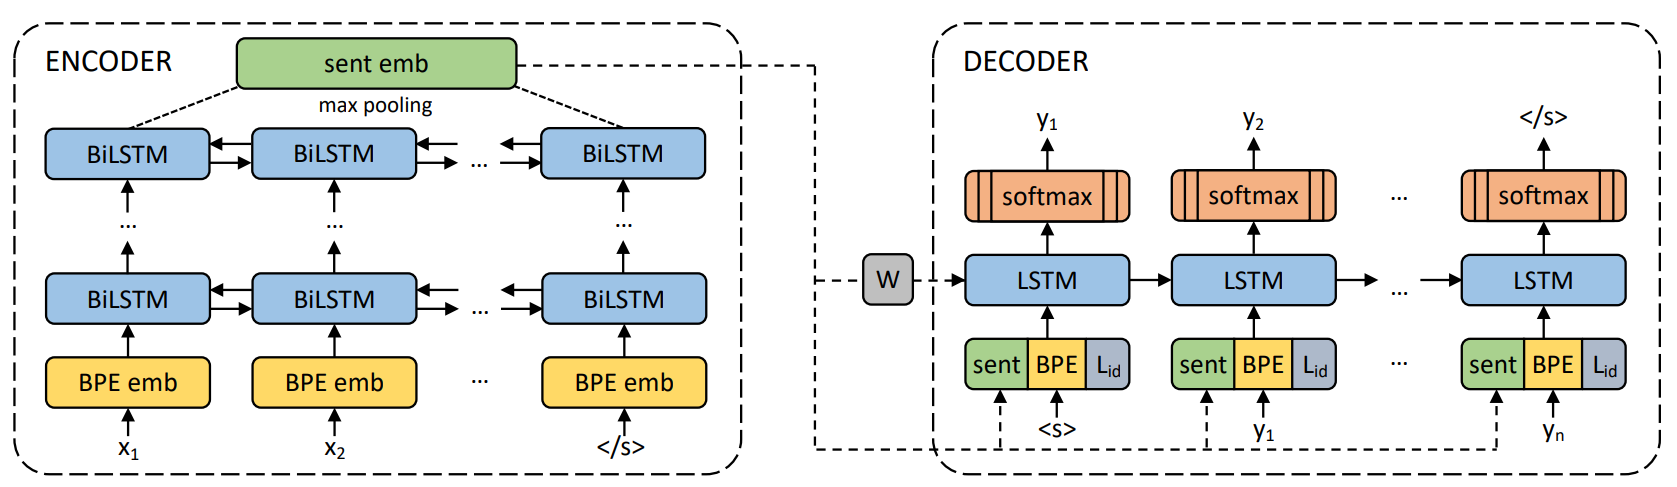
\includegraphics[scale=0.3]{images/laser_architecture}
	\caption[\textit{LASER} encoder architecture]
		{The architecture of the `massively multilingual sentence embeddings' which are part of the \textit{\gls{laser}} library.
		The image was taken from \citep{Artetxe.2018}.}
	\label{fig:laser_architecture}
\end{figure}

The sentence representation is then passed on to the decoder which generates a sequence of words similar to the \textit{Skip-Thought} approach. However, this model additionally gets a language flag as input indicating which language the decoder has to produce. With their approach the authors attempt to create \textbf{`universal language-agnostic sentence representations'}, i.\,e. the embeddings are designed to work well across many tasks and across multiple languages.

% -----------------------------------------------------------------------------------------------------------------------------------------------------
% Random Sentence Encoders
\subsubsection{Random Sentence Encoders}
\label{sec:rand_sent}

Recent research conducted by \citep{Wieting.2019} revealed that \textbf{random sentence representations provide a solid baseline} for more sophisticated algorithms. The authors investigate the results of several models whose parameters are chosen randomly without any training. It was found that while there is a gap between the performance of such random encoders and the representations generated by trained models, it is much smaller than one would expect. Three architectures are proposed in the paper: \ding{182} \textit{\gls{borep}}, \ding{183} \textit{random (Bi-)LSTMs} and \ding{184} \textit{\glspl{esn}} \citep{Jaeger.2001} out of which the first two are used in this thesis.

% -----------------------------------------------------------------------------------------------------------------------------------------------------
% Acquisition of Sentence Embeddings
\subsection{Acquisition of Sentence Embeddings}
\label{sec:sent_embs_acquisition}

Analogously to the previous chapter, it is useful to summarize the training details for all the sentence embeddings considered in the context of the experiments. Table \vref{tab:sent_emb_sources} gives an overview.

\highlight{Non-parameterized methods.} Recall, that non-parameterized methods do not require any training. Instead, they combine existing word embeddings (compositional models). The experiments will be conducted using all word embeddings discussed in section \vref{sec:word_embs} (\textit{word2vec}, \textit{FastText} and \textit{Attract-Repel}). All of these word embedding spaces have a dimensionality of 300 which entails that the sentence embeddings produced by the compositional models have the same dimensionality. An exception is the \textit{power means} embedding which is a concatenation of various means, where $p \in \{ -\infty, 0, 1, 2, +\infty \}$. Furthermore, the code for the \textit{hierarchical pooling} algorithm could not be found in the official repository, which is why it was implemented from scratch according to the paper. In the paper, a window size of $m = 5$ is used. Unfortunately, this information was discovered relatively late which is why the experiments were conducted with a different windows size of $m = 3$.

\highlight{Parameterized methods.} In the context of this thesis five trained parameterized methods are going to be evaluated: \textit{InferSent}, \textit{Quick-Thought}, \textit{sent2vec}, \textit{\gls{bert}} and \textit{\gls{laser}}. Furthermore, there are two types of random encoders: \textit{\gls{borep}} and the \textit{random \gls{bilstm}}. These random methods have parameters (parameterized method), but they are not trained after a random initialization. These models will (next to the majority class) serve as a baseline.

\textbf{Quick-Thought.} The \textit{Quick-Thought} models were trained on the Wikipedia dumps for the respective languages. The English model was also trained on Wikipedia and not downloaded from the official GitHub\github~ repository.\footnote{\url{https://github.com/lajanugen/S2V} (retrieved: September 04, 2019)} The reason for this is that there were some problems when trying to get the pre-trained model to work. Several issues regarding this problem have already been filed.\footnote{Cf. for example \url{https://github.com/lajanugen/S2V/issues/10} or \url{https://github.com/lajanugen/S2V/issues/8} \\ (retrieved: September 17, 2019)} Furthermore, for the Turkish and Georgian models, the number of epochs trained was increased, since there is considerably less data available for these languages.

\textbf{InferSent.} We trained the \textit{InferSent} models on the \gls{snli} data set. Unfortunately, this data set is originally only available for the English language. Therefore, the resources had to be translated. This was achieved using the Google translation \gls{api}. A major problem in this context was that the number of translation requests is limited. Only a certain number of requests per day are allowed. If this limit is exceeded, the server responds with \texttt{Error Code 500: Too many Requests} and one is blocked for 24\,h. In order to increase the speed, several sentences are concatenated which are jointly translated as a batch. Unfortunately, this entails that the translated sentences have to be mapped back to the original sentences (since the result returned is only one long string). It is crucial to assure that the number of sentences returned by the server is equal to the number of sentences fed into the translation procedure. If this is not the case, one risks that sentences and labels do not match anymore which would greatly impair the learning process.

In order to avoid this, the following strategy was employed: A special split token (a series of numbers) was introduced before concatenating the individual sentences in the original language. It was checked that this split token does not influence the quality of the translations in any harmful way. Further, the token was chosen such that it is not altered during the translation procedure (at least in the majority of the cases). When a translated batch arrives it is first split using this split token. The routine subsequently checks if this results in the expected number of sentences. If yes, the sentences are returned. If not, the split token is removed and the next attempt is to split at punctuation symbols (., !, ?). If this again fails, the sentences in that batch are translated one by one. The translations had to be done for Russian, Turkish and Georgian. A German translation of the \gls{snli} data set was already available.\footnote{\url{https://public.ukp.informatik.tu-darmstadt.de/arxiv2018-xling-sentence-embeddings/translated-snli/en-de-translated-snli-4x.zip} (retrieved: September 04, 2019)}

Since the translation procedure nonetheless took a very long time, it was not possible to translate all of the approximately 550,000 sentence pairs for each language, which is why the training set for the low-resource languages was restricted to 60,000 sentence pairs. All models employed use the \textit{InferSent2} version (using \textit{FastText} word embeddings) and the encoder architecture leveraged was the \gls{bilstm} with max-pooling, since this architecture achieved the best results in the experiments conducted by \citep{Conneau.2017}. Training the models takes a very long time. The time for training the German model was about 4 days. The English model was again available for download.\footnote{\url{https://github.com/facebookresearch/InferSent} (retrieved: September 04, 2019)}

% Table: Acquisition of sentence embeddings / models
\begin{table}
	\begin{adjustbox}{angle=90}
		\setlength{\fboxsep}{0pt}
\renewcommand{\arraystretch}{1.415}
\scalebox{1.0}{
\begin{tabularx}{0.935\textheight}{| c | l | p{0.6cm} | c | c | c | c | c | c | X |}
	\hline
	\cellcolor{tud9c!50}													&
	\cellcolor{tud9c!50}													&
	\cellcolor{tud9c!50}													&
	\cellcolor{tud9c!50}													&
	\cellcolor{tud9c!50}													&
	\multicolumn{5}{c |}{\cellcolor{tud9c!50}\textbf{Training details}} 		\\
	\cellcolor{tud9c!50}\multirow{-2}{*}{\textbf{Nr.}}						&
	\cellcolor{tud9c!50}\multirow{-2}{*}{\textbf{Embedding}}				&
	\cellcolor{tud9c!50}\multirow{-2}{*}{\textbf{Lng}}						&
	\cellcolor{tud9c!50}\multirow{-2}{*}{\textbf{Source}}					&
	\cellcolor{tud9c!50}\multirow{-2}{*}{\textbf{Word emb}}				&
	\cellcolor{tud9c!30}\textbf{dim}										&
	\cellcolor{tud9c!30}\textbf{\# instances} 								&
	\cellcolor{tud9c!30}\textbf{batch size} 									&
	\cellcolor{tud9c!30}\textbf{\# epochs} 									&
	\cellcolor{tud9c!30}\textbf{other params / comments}					\\
	\hline\hline
	\multicolumn{10}{| l |}{
		\cellcolor{tud9c!5}\textbf{Non-parameterized methods}}				\\ \hline

	% mean embeddings
	\circled{1} 															&
	\textit{Vanilla average}												&
	\AddCellBackground{0.6cm}{1.1\baselineskip}{images/flag_all}	 		&
	\faFilter																&
	\textit{all} 															&
	300																	&
	-		 															&
 	- 																	&
	- 																	&
	no training required													\\
	\hline

	% p-mean embeddings
	\circled{2} 															&
	\textit{$p$-means}													&
	\AddCellBackground{0.6cm}{1.1\baselineskip}{images/flag_all}	 		&
	\faFilter																&
	\textit{all} 															&
	1,500																	&
	-		 															&
 	- 																	&
	- 																	&
	no training required, $p \in \{ -\infty, 0, 1, 2, +\infty \}$								\\
	\hline

	% sif
	\circled{3} 															&
	\textit{\gls{sif}}														&
	\AddCellBackground{0.6cm}{1.1\baselineskip}{images/flag_all}	 		&
	\faFilter																&
	\textit{all} 															&
	300																	&
	-		 															&
 	- 																	&
	- 																	&
	no training required													\\
	\hline
	
	% gem
	\circled{4} 															&
	\textit{\gls{gem}}													&
	\AddCellBackground{0.6cm}{1.1\baselineskip}{images/flag_all}	 		&
	\faFilter																&
	\textit{all} 															&
	300																	&
	-		 															&
 	- 																	&
	- 																	&
	no training required													\\
	\hline

	% hier. pooling
	\circled{5} 															&
	\textit{hier. pooling}													&
	\AddCellBackground{0.6cm}{1.1\baselineskip}{images/flag_all}	 		&
	\faFilter																&
	\textit{all} 															&
	300																&
	-		 															&
 	- 																	&
	- 																	&
	no training required, window size $m = 3$										\\
	\hline\hline

	\multicolumn{10}{| l |}{
		\cellcolor{tud9c!5}\textbf{Parameterized methods}}					\\
	\hline

	% quickthought
	\circledBlk{1}														&
	\textit{Quick-Thought} 												&
	\AddCellBackground{0.6cm}{1.1\baselineskip}{images/flag_uk}	 		&
	\faCogs																&
	\textit{word2vec}														&
	2,400																&
	97,285,870															&
 	2,000 																&
	5 																	&
	-																	\\
	\hline

	\circledBlk{2}														&
	\textit{Quick-Thought} 												&
	\AddCellBackground{0.6cm}{1.1\baselineskip}{images/flag_germany}		&
	\faCogs																&
	\textit{word2vec} 													&
	2,400																&
	40,729,339 															&
 	1,000 																&
	5 																	&
	-																	\\
	\hline

	\circledBlk{3}														&
	\textit{Quick-Thought} 												&
	\AddCellBackground{0.6cm}{1.1\baselineskip}{images/flag_russia} 		&
	\faCogs																&
	\textit{word2vec} 													&
	2,400																&
	25,324,234		 													&
 	1,000																&
	5 																	&
	-																	\\
	\hline

	\circledBlk{4}														&
	\textit{Quick-Thought} 												&
	\AddCellBackground{0.6cm}{1.1\baselineskip}{images/flag_turkey} 		&
	\faCogs																&
	\textit{word2vec} 													&
	2,400																&
	3,797,955 															&
 	100 																&
	5 																	&
	-																	\\
	\hline

	\circledBlk{5}														&
	\textit{Quick-Thought} 												&
	\AddCellBackground{0.6cm}{1.1\baselineskip}{images/flag_georgia}		&
	\faCogs																&
	\textit{word2vec} 													&
	2,400																&
	1,047,780															&
 	100 																&
	12 																	&
																		\\
	\hline

	% infersent
	\circledBlk{6}														&
	\textit{InferSent} 														&
	\AddCellBackground{0.6cm}{1.1\baselineskip}{images/flag_uk}	 		&
	\faDownload															&
	\textit{FastText}															&
	4,096																&
	-		 															&
 	- 																	&
	- 																	&
	Version: \textit{infersent2}	, max-pooling, model:
	\href{https://dl.fbaipublicfiles.com/infersent/infersent2.pkl}
		{\linkstyle{Link}}													\\
	\hline

	\circledBlk{7}														&
	\textit{InferSent} 														&
	\AddCellBackground{0.6cm}{1.1\baselineskip}{images/flag_germany}		&
	\faCogs																&
	\textit{FastText}														&
	4,096																&
	547,743		 														&
 	64 																	&
	10 																	&
	Version: \textit{infersent2}	, max-pooling								\\
	\hline

	\circledBlk{8}														&
	\textit{InferSent} 														&
	\AddCellBackground{0.6cm}{1.1\baselineskip}{images/flag_russia}		&
	\faCogs																&
	\textit{FastText}														&
	4,096																&
	60,000	 															&
 	64 																	&
	15 																	&
	Version: \textit{infersent2}	, max-pooling								\\
	\hline

	\circledBlk{9}														&
	\textit{InferSent} 														&
	\AddCellBackground{0.6cm}{1.1\baselineskip}{images/flag_turkey} 		&
	\faCogs																&
	\textit{FastText}														&
	4,096																&
	60,000	 															&
 	64 																	&
	15 																	&
	Version: \textit{infersent2}	, max-pooling								\\
	\hline

	\circledBlk{10}														&
	\textit{InferSent} 														&
	\AddCellBackground{0.6cm}{1.1\baselineskip}{images/flag_georgia}		&
	\faCogs																&
	\textit{FastText}														&
	4,096																&
	60,000	 															&
 	64 																	&
	15 																	&
	Version: \textit{infersent2}	, max-pooling								\\
	\hline

	% sent2vec
	\circledBlk{11}														&
	\textit{sent2vec} 														&
	\AddCellBackground{0.6cm}{1.1\baselineskip}{images/flag_uk}	 		&
	\faDownload															&
	\textit{FastText}														&
	700																	&
	-		 															&
 	- 																	&
	- 																	&
	model: \texttt{sent2vec\_wiki\_bigrams},
	\href{https://drive.google.com/file/d/0B6VhzidiLvjSaER5YkJUdWdPWU0/view}
		{\linkstyle{Link}}													\\
	\hline

	\circledBlk{12}														&
	\textit{sent2vec} 														&
	\AddCellBackground{0.6cm}{1.1\baselineskip}{images/flag_germany}		&
	\faCogs																&
	\textit{FastText}														&
	700																	&
	40,729,339		 													&
 	- 																	&
	9 																	&
	\texttt{lr}: 0.2, \texttt{wordNgrams}: 2,
		\texttt{neg}: 10, \texttt{dropoutK}: 4								\\
	\hline

	\circledBlk{13}														&
	\textit{sent2vec} 														&
	\AddCellBackground{0.6cm}{1.1\baselineskip}{images/flag_russia} 		&
	\faCogs																&
	\textit{FastText}														&
	700																	&
	25,324,234		 													&
 	- 																	&
	9 																	&
	\texttt{lr}: 0.2, \texttt{wordNgrams}: 2,
		\texttt{neg}: 10, \texttt{dropoutK}: 4								\\
	\hline

	\circledBlk{14}														&
	\textit{sent2vec} 														&
	\AddCellBackground{0.6cm}{1.1\baselineskip}{images/flag_turkey}		&
	\faCogs																&
	\textit{FastText}														&
	700																	&
	3,797,955		 													&
 	- 																	&
	9 																	&
	\texttt{lr}: 0.2, \texttt{wordNgrams}: 2,
		\texttt{neg}: 10, \texttt{dropoutK}: 4								\\
	\hline

	\circledBlk{15}														&
	\textit{sent2vec} 														&
	\AddCellBackground{0.6cm}{1.1\baselineskip}{images/flag_georgia}		&
	\faCogs																&
	\textit{FastText}														&
	700																	&
	1,047,780		 													&
 	- 																	&
	9 																	&
	\texttt{lr}: 0.2, \texttt{wordNgrams}: 2,
		\texttt{neg}: 10, \texttt{dropoutK}: 4								\\
	\hline

	% bert
	\circledBlk{16}														&
	\textit{\gls{bert}} 													&
	\AddCellBackground{0.6cm}{1.1\baselineskip}{images/flag_all}	 		&
	\faDownload															&
	-																	&
	768																	&
	-		 															&
 	- 																	&
	- 																	&
	multilingual model:
	\href{https://storage.googleapis.com/bert_models/2018_11_23/multi_cased_L-12_H-768_A-12.zip}
		{\linkstyle{Link}}													\\
	\hline

	% laser
	\circledBlk{17}														&
	\textit{\gls{laser}}													&
	\AddCellBackground{0.6cm}{1.1\baselineskip}{images/flag_all}	 		&
	\faDownload															&
	-																	&
	1,024 																&
	-		 															&
 	- 																	&
	- 																	&
	multilingual model:
	\href{https://github.com/facebookresearch/LASER}
	{\linkstyle{Link}}														\\
	\hline

	% random sentence encoder - borep
	\circledBlk{18}														&
	\textit{RandSent \gls{borep}} 											&
	\AddCellBackground{0.6cm}{1.1\baselineskip}{images/flag_all}	 		&
	\faMagic																&
	\textit{FastText}														&
	4,096																&
	-		 															&
 	- 																	&
	- 																	&
	-																	\\
	\hline

	% random sentence encoder - lstm
	\circledBlk{19}														&
	\textit{RandSent \gls{bilstm}} 											&
	\AddCellBackground{0.6cm}{1.1\baselineskip}{images/flag_all}	 		&
	\faMagic																&
	\textit{FastText}														&
	8,192																&
	-		 															&
 	- 																	&
	- 																	&
	-																	\\
	\hline
\end{tabularx}}
	\end{adjustbox}
	\vspace*{-5mm}
	\caption[Sources of sentence embeddings]
		{Overview of sentence embedding acquisition separated by non-parametric and parametric approaches.
		Legend: \faFilter\ Compositional methods, \faDownload\ downloaded models, \faCogs\ trained models,
		\faMagic\ random encoders}
	\label{tab:sent_emb_sources}
\end{table}

\textbf{sent2vec.} The models for the \textit{sent2vec} approach were trained on Wikipedia (German, Russian, Turkish and Georgian). The values for the hyper-parameters can be read off from table \vref{tab:sent_emb_sources}. The training procedure was rather fast. The English model was downloaded using a link from GitHub\github.\footnote{\url{https://github.com/epfml/sent2vec} (retrieved: September 04, 2019)}

\textbf{\gls{bert}.} Training \textit{\gls{bert}} is only possible if one has a \gls{tpu} at one's disposal. This was not the case. But a multilingual model is offered on GitHub\github.\footnote{\url{https://github.com/google-research/bert/blob/master/multilingual.md} (retrieved: September 04, 2019)} The model used is called \texttt{\gls{bert}-Base, Multilingual Cased}. It is applicable to 104 languages and has about 110 million parameters.

\textbf{\gls{laser}.} The model is multilingual and available in pre-trained form. It was downloaded and installed following the instructions on GitHub\github.\footnote{\url{https://github.com/facebookresearch/LASER} (retrieved: September 04, 2019)}

% -----------------------------------------------------------------------------------------------------------------------------------------------------
% Chapter Summary
\subsection{Summary}
\label{sec:sent_embs_summary}

This chapter introduced several sentence embedding algorithms. Generally speaking, there is a distinction between non-parameterized and parameterized sentence embeddings. The first kind of algorithms makes use of word embeddings as a basis and perform some kind of pooling operation in order to obtain a sentence embedding. The more sophisticated parameterized models which are often realized using neural architectures train sentence embeddings from scratch either in an unsupervised or supervised fashion.

The final section then gave insights into the process of sentence embedding acquisition. Models for the English language were mostly found to be publicly accessible in a pre-trained manner and were therefore downloaded from the official websites. Especially models for the low-resource languages Russian, Turkish and Georgian were not available which is why we had to train them from scratch (\textit{sent2vec}, \textit{Quick-Thought} and \textit{InferSent}).
